\chapter{Symétrie et lois de conservation}

\lectureoverview{L’action stationnaire et les équations d’Euler--Lagrange constituent une moitié du cœur de la mécanique classique ; la formulation hamiltonienne en est l’autre. Nous allons développer suffisamment cette première moitié pour mettre au jour un schéma profond : toute symétrie continue d’un lagrangien produit une grandeur conservée. Nous découvrirons ce schéma à travers les translations et les rotations, le démontrerons pour une transformation infinitésimale générale, puis examinerons avec soin les cas où le raisonnement s’applique et ceux où il ne s’applique pas.}

\section{Le minimum de mathématiques qui explique la physique}

Les expressions déjà inscrites au tableau ressemblent peut-être un peu à l’équation de Schrödinger, mais ce n’est pas le sujet de ce soir. Nous allons parler de symétrie et de conservation. Il est impossible d’expliquer honnêtement leur lien sans équations. Les équations sont élémentaires ; l’essentiel est de les agencer de façon à faire apparaître la structure. Scientific American peut nommer le résultat, mais nous voulons ici établir le minimum de mathématiques nécessaire pour le déduire comme le feraient des physiciens.

Introduisons un petit paramètre \(\epsilon\). Nous conservons les termes proportionnels à \(\epsilon\) et négligeons ceux en \(O(\epsilon^2)\). C’est une façon abrégée de désigner un raisonnement par passage à la limite, et non d’affirmer que le carré d’un nombre réel non nul est littéralement nul. Pour une fonction ordinaire \(f(x,y)\),
\begin{equation}
  \delta f
  =\frac{\partial f}{\partial x}\,\delta x
   +\frac{\partial f}{\partial y}\,\delta y
   +O(\epsilon^2),
  \label{eq:first-variation-f}
\end{equation}
où \(\delta x\) et \(\delta y\) sont toutes deux proportionnelles à \(\epsilon\). Le symbole \(\delta f\) désigne la variation de \(f\), et non le produit d’un nombre appelé \(\delta\) par \(f\). Un point stationnaire vérifie
\begin{equation}
  \delta f=0
  \qquad\hbox{to first order.}
  \label{eq:stationary-f}
\end{equation}

Pour une trajectoire mécanique \(q_i(t)\), la quantité analogue est l’action
\begin{equation}
  S[q]=\int_{t_1}^{t_2}L(q,\dot q,t)\,dt.
  \label{eq:action-l4}
\end{equation}
La variation de la trajectoire à extrémités fixes donne
\begin{equation}
  \delta S
  =\int_{t_1}^{t_2}dt\,
   \sum_i\left(
     \frac{\partial L}{\partial q_i}\,\delta q_i
     +\frac{\partial L}{\partial\dot q_i}\,\delta\dot q_i
   \right).
  \label{eq:action-variation-l4}
\end{equation}
Les deux termes apparaissent parce qu’une variation de trajectoire modifie à la fois sa position et sa vitesse. L’intégration par parties, associée à
\(\delta q_i(t_1)=\delta q_i(t_2)=0\), transforme \(\delta S=0\) en
\begin{equation}
  \frac{d}{dt}\left(\frac{\partial L}{\partial\dot q_i}\right)
  -\frac{\partial L}{\partial q_i}=0.
  \label{eq:el-l4}
\end{equation}

\begin{figure}[htbp]
  \centering
  \includegraphics[width=0.76\textwidth]{lecture_04_figure_05.png}
  \caption{L’équation d’Euler--Lagrange, rappelée comme point de départ pour étudier symétrie et conservation.}
  \lectureframe{00:09:00}
\end{figure}

L’expression correcte est \emph{action stationnaire}, et non nécessairement action minimale. Nous reviendrons sur cette distinction vers la fin.

\section{Coordonnées généralisées et quantité de mouvement conjuguée}

Les positions cartésiennes ne suffisent pas à décrire la mécanique générale. Les coordonnées peuvent être des positions de particules, des angles, des variables collectives ou des amplitudes de champ ; nous les appelons donc \(q_i\). Un lagrangien est une description condensée de la dynamique. Même le Modèle standard, écrit sans notation très condensée, occupe environ une page ; écrire une équation du mouvement distincte pour chaque composante de champ en demanderait beaucoup plus. La fonction unique \(L\) rassemble toutes ces informations.

La quantité de mouvement conjuguée à \(q_i\) est
\begin{equation}
  p_i=\frac{\partial L}{\partial\dot q_i}.
  \label{eq:canonical-momentum-l4}
\end{equation}
C’est pourquoi on appelle traditionnellement les coordonnées généralisées des \(q\) ; les quantités de mouvement correspondantes sont des \(p\), ce qui nous donne nos \(p\) et nos \(q\). Avec cette notation, l’équation ~\eqref{eq:el-l4} devient
\begin{equation}
  \dot p_i=\frac{\partial L}{\partial q_i}.
  \label{eq:momentum-el-l4}
\end{equation}

Pour la particule familière à une dimension,
\begin{equation}
  L=\frac{m\dot x^2}{2}-V(x),
  \qquad
  \frac{\partial L}{\partial\dot x}=m\dot x,
  \label{eq:particle-momentum-l4}
\end{equation}
la quantité de mouvement conjuguée est donc la quantité de mouvement ordinaire.

\begin{figure}[htbp]
  \centering
  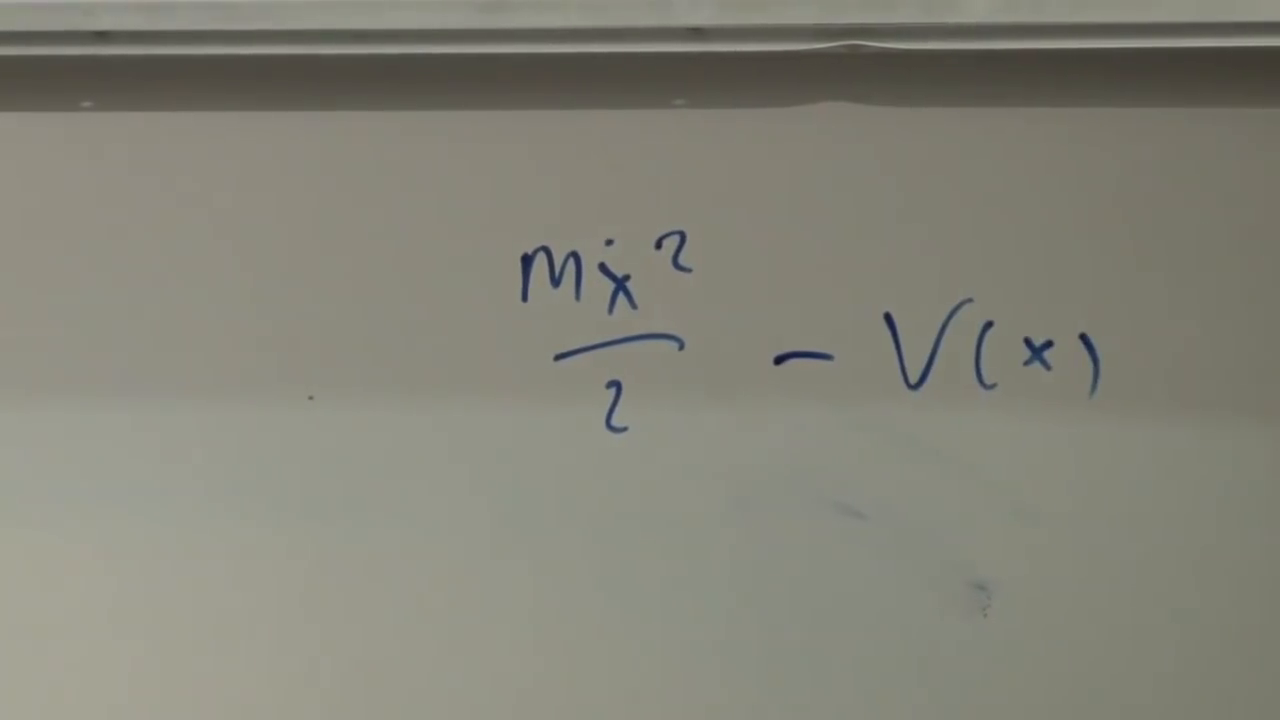
\includegraphics[width=0.72\textwidth]{lecture_04_figure_02.png}
  \caption{Le lagrangien égal à l’énergie cinétique moins l’énergie potentielle, utilisé pour identifier la quantité de mouvement conjuguée à \(m\dot x\).}
  \lectureframe{00:14:48}
\end{figure}

Si \(q_i\) n’apparaît pas dans \(L\), alors \(\dot p_i=0\). C’est la démarche familière qui consiste à invoquer une coordonnée cyclique pour obtenir une loi de conservation. Le lien véritable est plus général, et il est utile de le découvrir à travers des exemples avant de le démontrer.

\section{Découvrir des lois de conservation avant de les expliquer}

\subsection{Deux coordonnées et un potentiel dépendant de leur écart}

Prenons les deux masses égales à l’unité et considérons
\begin{equation}
  L=\frac{\dot q_1^{\,2}+\dot q_2^{\,2}}{2}-V(q_1-q_2).
  \label{eq:separation-lagrangian}
\end{equation}
On peut se représenter deux particules sur une droite. Leur interaction ne dépend que de leur écart.

\begin{figure}[htbp]
  \centering
  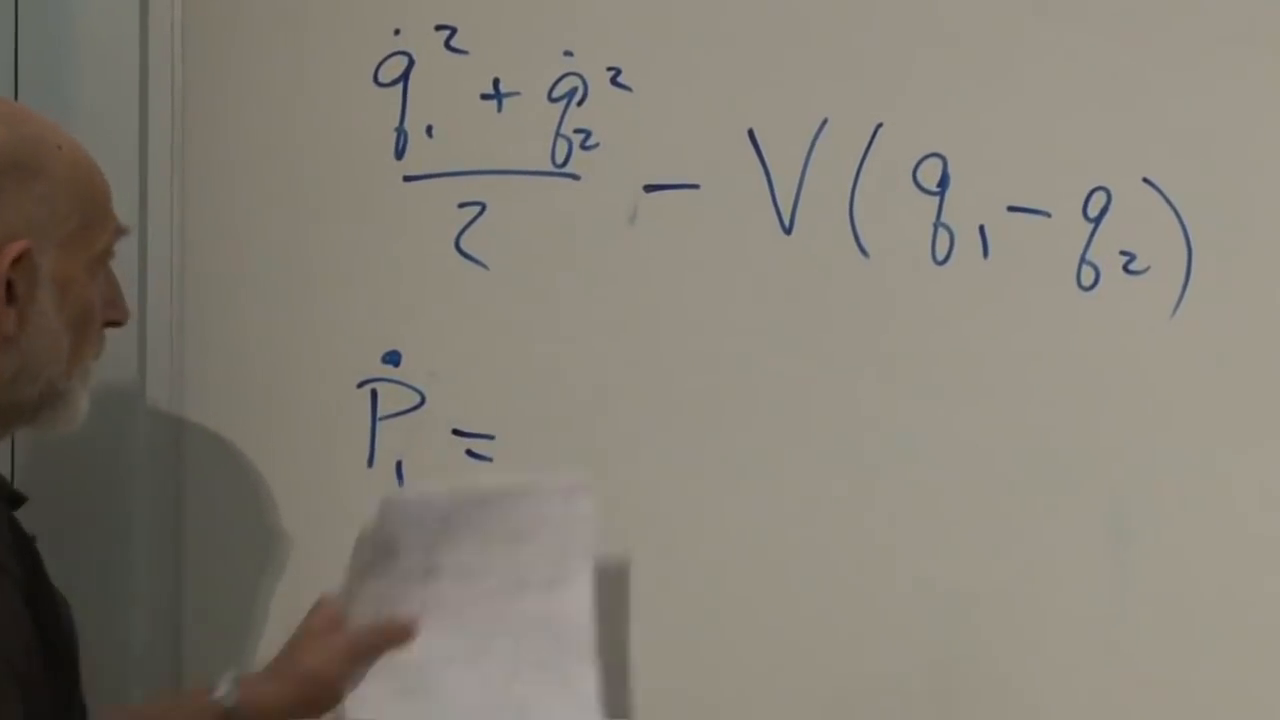
\includegraphics[width=0.78\textwidth]{lecture_04_figure_03.png}
  \caption{Le lagrangien à deux coordonnées et le début de la première équation pour les quantités de mouvement.}
  \lectureframe{00:18:56}
\end{figure}

Notons \(V'\) la dérivée par rapport à l’argument de \(V\) ; on obtient
\begin{align}
  \dot p_1&=-V'(q_1-q_2),
  \notag\\
  \dot p_2&=+V'(q_1-q_2).
  \label{eq:separation-momentum-equations}
\end{align}
Le signe de la seconde équation est opposé parce qu’une augmentation de \(q_2\) diminue \(q_1-q_2\).

\begin{classroomqa}
  \audiencequestion{La première équation pour la quantité de mouvement doit-elle contenir \(V'\), et d’où vient son signe moins ?
  \lecturetimestamp{00:20:52--00:21:35}}
  \lecturerresponse{L’équation d’Euler--Lagrange indique que
  \(\dot p_1=\partial L/\partial q_1\), et non que le lagrangien est nul.
  Puisque \(L=T-V\), la dérivation par rapport à \(q_1\) donne
  \(-V'\). La dérivation par rapport à \(q_2\) ajoute un autre signe moins, provenant de \(q_1-q_2\) ; la seconde équation contient donc \(+V'\).}
\end{classroomqa}

\begin{figure}[htbp]
  \centering
  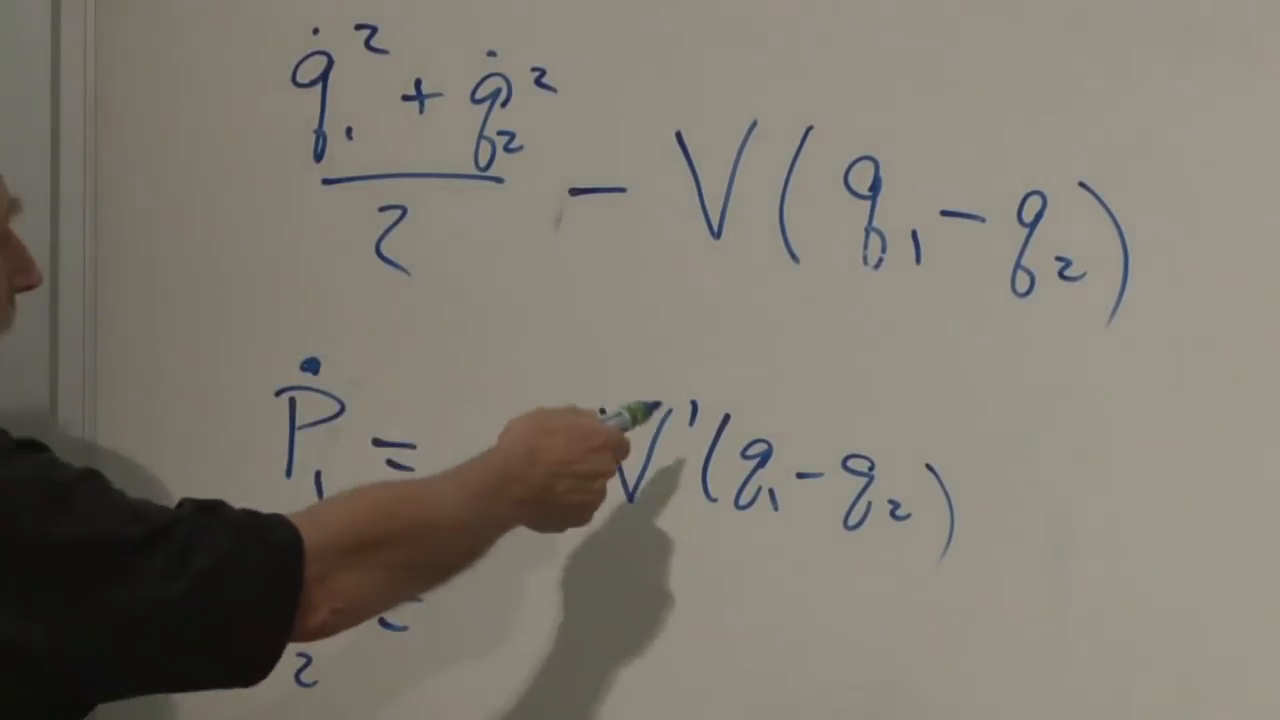
\includegraphics[width=0.78\textwidth]{lecture_04_figure_04.png}
  \caption{La dérivée dont le signe est crucial dans l’équation de \(p_1\) ; l’équation de \(p_2\) reçoit le signe opposé.}
  \lectureframe{00:20:41}
\end{figure}

En additionnant les équations ~\eqref{eq:separation-momentum-equations}, on obtient
\begin{equation}
  \frac{d}{dt}(p_1+p_2)=0.
  \label{eq:total-p-conserved}
\end{equation}
Nous avons trouvé une grandeur conservée, sans encore expliquer pourquoi elle existe.

\subsection{Une combinaison linéaire moins évidente}

Posons maintenant
\begin{equation}
  L=\frac{\dot q_1^{\,2}+\dot q_2^{\,2}}{2}
    -V(Aq_1+Bq_2),
  \label{eq:ab-lagrangian}
\end{equation}
où \(A\) et \(B\) sont des constantes. Alors
\begin{align}
  \dot p_1&=-A\,V'(Aq_1+Bq_2),
  \notag\\
  \dot p_2&=-B\,V'(Aq_1+Bq_2).
  \label{eq:ab-momentum-equations}
\end{align}
En multipliant la première équation par \(B\), la seconde par \(A\), puis en soustrayant, on élimine la force :
\begin{equation}
  \frac{d}{dt}(Bp_1-Ap_2)=0.
  \label{eq:ab-conserved}
\end{equation}

\begin{figure}[htbp]
  \centering
  \includegraphics[width=0.78\textwidth]{lecture_04_figure_06.png}
  \caption{Les équations pondérées pour les quantités de mouvement, dont les termes de force s’annulent dans \(Bp_1-Ap_2\).}
  \lectureframe{00:24:20}
\end{figure}

\begin{classroomqa}
  \audiencequestion{Quelle interprétation physique peut-on donner à des constantes telles que \(A\) et \(B\) ?
  \lecturetimestamp{00:25:09--00:30:15}}
  \lecturerresponse{Considérons deux particules de masses \(m\) et \(M\) :
  \[
    L=\frac{m\dot X^2}{2}+\frac{M\dot Y^2}{2}-V(X-Y).
  \]
  Faisons le changement d’échelle \(Q_1=\sqrt m\,X\) et \(Q_2=\sqrt M\,Y\). Le terme cinétique devient \((\dot Q_1^2+\dot Q_2^2)/2\), tandis que le potentiel dépend de \(Q_1/\sqrt m-Q_2/\sqrt M\). Ainsi, des masses inégales deviennent naturellement des coefficients dans une combinaison linéaire. Remplacer \(Q_2\) par \(-Q_2\) transforme le signe moins affiché en signe plus, sans modifier le terme cinétique quadratique.}
\end{classroomqa}

\begin{figure}[htbp]
  \centering
  \includegraphics[width=0.82\textwidth]{lecture_04_figure_07.png}
  \caption{Les coordonnées pondérées par les masses simplifient l’énergie cinétique, tandis que les facteurs de masse se retrouvent dans le potentiel.}
  \lectureframe{00:28:40}
\end{figure}

\begin{classroomqa}
  \audiencequestion{Cela montre-t-il qu’une grandeur conservée peut exister sans coordonnée cyclique ?
  \lecturetimestamp{00:31:13--00:31:58}}
  \lecturerresponse{Dans les variables écrites ici, il n’y a pas de coordonnée cyclique \emph{évidente}. Un changement de variables peut en faire apparaître une, mais ce n’est pas la façon utile d’aborder le problème que de la rechercher. L’argument de symétrie identifiera directement la combinaison conservée.}
\end{classroomqa}

\section{Ce que nous entendons par symétrie}

\subsection{Translations}

Partons d’une particule libre de masse unité,
\begin{equation}
  L=\frac{\dot q^2}{2}.
  \label{eq:free-unit-l4}
\end{equation}
Translatons chaque point de son histoire de la même constante :
\begin{equation}
  q'(t)=q(t)+\epsilon.
  \label{eq:free-translation}
\end{equation}
Comme \(\epsilon\) ne dépend pas du temps, \(\dot q'=\dot q\), et donc
\(\delta L=0\). Cette invariance est une symétrie de translation.

Il existe deux descriptions équivalentes. Dans la description passive, on déplace l’origine des coordonnées en laissant l’objet fixe. Dans la description active, on garde les axes fixes et on déplace l’objet. Le langage actif sera moins source de confusion : déplaçons la configuration physique et demandons-nous si \(L\) s’en aperçoit.

Pour l’équation ~\eqref{eq:separation-lagrangian}, translatons les deux coordonnées :
\begin{equation}
  \delta q_1=\epsilon,
  \qquad
  \delta q_2=\epsilon.
  \label{eq:common-translation}
\end{equation}
Les vitesses restent inchangées, tout comme \(q_1-q_2\).

\begin{figure}[htbp]
  \centering
  \includegraphics[width=0.78\textwidth]{lecture_04_figure_08.png}
  \caption{Une translation commune laisse inchangé l’écart entre deux coordonnées.}
  \lectureframe{00:35:30}
\end{figure}

Pour l’équation ~\eqref{eq:ab-lagrangian}, considérons la transformation moins évidente
\begin{equation}
  \delta q_1=B\epsilon,
  \qquad
  \delta q_2=-A\epsilon.
  \label{eq:ab-transformation}
\end{equation}
Là encore, les vitesses ne changent pas, tandis que
\begin{equation}
  \delta(Aq_1+Bq_2)=AB\epsilon-BA\epsilon=0.
  \label{eq:ab-invariant-argument}
\end{equation}
Cette transformation est donc une symétrie.

\begin{figure}[htbp]
  \centering
  \includegraphics[width=0.80\textwidth]{lecture_04_figure_09.png}
  \caption{La translation asymétrique qui préserve \(Aq_1+Bq_2\).}
  \lectureframe{00:40:20}
\end{figure}

\begin{classroomqa}
  \audiencequestion{Les coefficients représentent-ils les masses, de sorte que la grandeur conservée devienne la quantité de mouvement ordinaire du centre de masse ?
  \lecturetimestamp{00:42:25--00:42:45}}
  \lecturerresponse{Oui. Dans les variables pondérées par les masses, la symétrie et la combinaison conservée semblent asymétriques. En revenant à \(X\) et \(Y\), on retrouve la translation simultanée ordinaire et la quantité de mouvement totale.}
\end{classroomqa}

\subsection{Rotations}

Considérons une particule dans le plan,
\begin{equation}
  L=\frac{m}{2}(\dot x^2+\dot y^2)-V(x^2+y^2).
  \label{eq:central-lagrangian-l4}
\end{equation}
Il s’agit d’un potentiel central. Comparons deux systèmes de coordonnées fixes, tournés l’un par rapport à l’autre ; les axes ne tournent pas au cours du temps. En choisissant une orientation cohérente,
\begin{align}
  x'&=x\cos\theta+y\sin\theta,
  \notag\\
  y'&=-x\sin\theta+y\cos\theta.
  \label{eq:finite-rotation-l4}
\end{align}

\begin{figure}[htbp]
  \centering
  \includegraphics[width=0.82\textwidth]{lecture_04_figure_10.png}
  \caption{Un lagrangien à potentiel central et deux repères cartésiens fixes liés par une rotation.}
  \lectureframe{00:45:40}
\end{figure}

Posons \(\theta=\epsilon\) et conservons les termes du premier ordre :
\begin{equation}
  \cos\epsilon=1+O(\epsilon^2),
  \qquad
  \sin\epsilon=\epsilon+O(\epsilon^3).
  \label{eq:small-angle-l4}
\end{equation}
La rotation infinitésimale s’écrit
\begin{align}
  \delta x&=y\epsilon,
  &\delta y&=-x\epsilon,
  \notag\\
  \delta\dot x&=\dot y\epsilon,
  &\delta\dot y&=-\dot x\epsilon.
  \label{eq:infinitesimal-rotation-l4}
\end{align}

\begin{figure}[htbp]
  \centering
  \includegraphics[width=0.82\textwidth]{lecture_04_figure_11.png}
  \caption{La rotation infinitésimale des coordonnées et des vitesses.}
  \lectureframe{00:49:50}
\end{figure}

À la différence d’une translation, la variation de \(x\) dépend de \(y\), et celle de \(y\) dépend de \(x\). Pourtant,
\begin{align}
  \delta(x^2+y^2)
  &=2x\,\delta x+2y\,\delta y=0,
  \notag\\
  \delta(\dot x^2+\dot y^2)
  &=2\dot x\,\delta\dot x+2\dot y\,\delta\dot y=0.
  \label{eq:rotation-invariants-l4}
\end{align}
Les termes de potentiel et d’énergie cinétique sont tous deux invariants.

\begin{figure}[htbp]
  \centering
  \includegraphics[width=0.76\textwidth]{lecture_04_figure_12.png}
  \caption{L’annulation au premier ordre qui démontre l’invariance du rayon au carré par rotation.}
  \lectureframe{00:53:20}
\end{figure}

\section{Théorème général de conservation}

Les exemples de translation et de rotation ont la même forme. Considérons une transformation continue infinitésimale
\begin{equation}
  \delta q_i=\epsilon f_i(q),
  \qquad
  \delta\dot q_i=\frac{d}{dt}\delta q_i,
  \label{eq:general-infinitesimal-symmetry}
\end{equation}
où \(\epsilon\) est indépendant du temps et où \(f_i\) peut dépendre de toutes les coordonnées.

\begin{figure}[htbp]
  \centering
  \includegraphics[width=0.78\textwidth]{lecture_04_figure_13.png}
  \caption{Un champ général de déplacements infinitésimaux \(\delta q_i=\epsilon f_i(q)\).}
  \lectureframe{00:56:00}
\end{figure}

La variation du lagrangien au premier ordre est
\begin{equation}
  \delta L
  =\sum_i\left(
    \frac{\partial L}{\partial q_i}\delta q_i
    +\frac{\partial L}{\partial\dot q_i}\delta\dot q_i
  \right).
  \label{eq:delta-l-general}
\end{equation}

\begin{figure}[htbp]
  \centering
  \includegraphics[width=0.84\textwidth]{lecture_04_figure_14.png}
  \caption{Les deux contributions à \(\delta L\) : la variation des coordonnées et celle des vitesses.}
  \lectureframe{01:02:30}
\end{figure}

Restreignons-nous maintenant à une trajectoire physique, qui vérifie donc les équations d’Euler--Lagrange. En utilisant
\begin{equation}
  \frac{\partial L}{\partial\dot q_i}=p_i,
  \qquad
  \frac{\partial L}{\partial q_i}=\dot p_i,
  \label{eq:el-substitution-l4}
\end{equation}
on trouve
\begin{align}
  \delta L
  &=\sum_i\left(\dot p_i\,\delta q_i
                +p_i\,\delta\dot q_i\right)
  \notag\\
  &=\frac{d}{dt}\sum_i p_i\delta q_i
  =\epsilon\frac{d}{dt}\sum_i p_i f_i(q).
  \label{eq:noether-derivation-l4}
\end{align}
L’étape centrale consiste simplement à appliquer la règle du produit.

Si la transformation est une symétrie, alors \(\delta L=0\). Comme \(\epsilon\) est un facteur constant arbitraire,
\begin{equation}
  \boxed{
  \frac{d\mathcal Q}{dt}=0,
  \qquad
  \mathcal Q=\sum_i p_i f_i(q)}
  .
  \label{eq:noether-charge-l4}
\end{equation}
C’est le cœur, en mécanique classique, du théorème de Noether pour les symétries ponctuelles exactes et indépendantes du temps.

\begin{figure}[htbp]
  \centering
  \includegraphics[width=0.84\textwidth]{lecture_04_figure_15.png}
  \caption{L’étape où la règle du produit transforme l’invariance de \(L\) en une grandeur conservée.}
  \lectureframe{01:05:00}
\end{figure}

\begin{classroomqa}
  \audiencequestion{Dans \(f_i(q)\), \(q\) comporte-t-il un autre indice ?
  \lecturetimestamp{01:06:57--01:07:31}}
  \lecturerresponse{Le symbole \(q\) sans indice désigne l’ensemble entier \((q_1,q_2,\ldots)\). Chaque composante \(f_i\) peut dépendre de toutes ces coordonnées. Dans le cas d’une rotation, par exemple, \(f_x=y\) et \(f_y=-x\).}
\end{classroomqa}

Les exemples cessent alors d’être de simples coïncidences. Pour une translation commune, on a \(f_1=f_2=1\), donc
\begin{equation}
  \mathcal Q=p_1+p_2.
  \label{eq:noether-common-p}
\end{equation}
Pour la translation asymétrique, on a \(f_1=B\), \(f_2=-A\), donc
\begin{equation}
  \mathcal Q=Bp_1-Ap_2.
  \label{eq:noether-ab-p}
\end{equation}
Pour une rotation, \(f_x=y\) et \(f_y=-x\) :
\begin{equation}
  \mathcal Q=p_xy-p_yx.
  \label{eq:rotation-charge-sign}
\end{equation}
Au signe d’orientation près, il s’agit du moment cinétique,
\begin{equation}
  J=xp_y-yp_x.
  \label{eq:angular-momentum-l4}
\end{equation}

\begin{figure}[htbp]
  \centering
  \includegraphics[width=0.82\textwidth]{lecture_04_figure_16.png}
  \caption{La charge de Noether associée à la rotation, égale au moment cinétique plan à un signe d’orientation près.}
  \lectureframe{01:11:00}
\end{figure}

Pour plusieurs particules en interaction, faisons tourner toutes les particules ensemble. L’invariance implique alors la conservation de la somme de leurs moments cinétiques, et non de celui de chaque particule prise séparément.

\section{Questions sur les hypothèses du théorème}

\begin{classroomqa}
  \audiencequestion{Un repère en rotation introduirait-il une dépendance explicite en temps dans \(\delta L\) ?\lecturetimestamp{01:12:57--01:13:57}}
  \lecturerresponse{Oui. La démonstration qui précède suppose un paramètre de symétrie indépendant du temps : une translation fixe ou une rotation fixe. Une transformation dont le paramètre dépend du temps produit des termes supplémentaires et exige un traitement plus général.}
\end{classroomqa}

\begin{classroomqa}
  \audiencequestion{Dans la formule au tableau, la lettre majuscule \(Q\) désigne-t-elle la transformation elle-même ?
  \lecturetimestamp{01:14:02--01:15:58}}
  \lecturerresponse{Non. Cette notation entre malheureusement en conflit avec les coordonnées \(q_i\). La transformation est \(\delta q_i=\epsilon f_i(q)\) ; la grandeur conservée qui en résulte est \(\mathcal Q=\sum_i p_i f_i\). Le coefficient \(f_i\) indique comment la coordonnée d’indice \(i\) se déplace sous l’effet de la symétrie.}
\end{classroomqa}

La conservation de l’énergie est elle aussi engendrée par une symétrie, mais d’une autre nature : la translation dans le temps, ou l’indépendance vis-à-vis du choix de l’origine des temps. Nous remettons à plus tard l’étude de ce cas et de la formulation hamiltonienne.

\begin{classroomqa}
  \audiencequestion{Le mouvement réel pourrait-il être absorbé dans un système de coordonnées variable, de sorte que la mécanique ne soit plus qu’un ensemble de transformations de coordonnées ?
  \lecturetimestamp{01:17:43--01:20:01}}
  \lecturerresponse{On peut choisir des coordonnées qui suivent un mouvement donné, mais la transformation dépend alors de l’état initial et de la trajectoire. La transformation de symétrie utilisée ici est fixée indépendamment de la solution suivie par le système. Le mouvement lui-même se représente plus naturellement dans l’espace combiné des coordonnées et des quantités de mouvement.}
\end{classroomqa}

\section{L’oscillateur harmonique dans l’espace des phases}

Prenons la masse et la constante de raideur égales à l’unité,
\begin{equation}
  L=\frac{\dot q^2}{2}-\frac{q^2}{2}.
  \label{eq:oscillator-l4}
\end{equation}
La quantité de mouvement conjuguée et l’équation du mouvement donnent
\begin{equation}
  p=\dot q,
  \qquad
  \dot p=-q,
  \label{eq:oscillator-first-order-l4}
\end{equation}
ou encore
\begin{equation}
  \dot q=p,
  \qquad
  \dot p=-q.
  \label{eq:oscillator-phase-flow}
\end{equation}
Ces équations décrivent un mouvement circulaire uniforme dans le plan \(q\)-\(p\). L’oscillation de va-et-vient dans l’espace réel est la projection de ce cercle sur l’axe \(q\) : la vitesse est maximale en \(q=0\) et s’annule aux points de rebroussement.

\begin{figure}[htbp]
  \centering
  \includegraphics[width=0.82\textwidth]{lecture_04_figure_17.png}
  \caption{Les équations de l’oscillateur harmonique et son orbite circulaire dans l’espace \(q\)-\(p\).}
  \lectureframe{01:25:30}
\end{figure}

\begin{classroomqa}
  \audiencequestion{Le cercle dans l’espace des phases est-il parcouru dans le sens horaire ?
  \lecturetimestamp{01:25:47--01:27:15}}
  \lecturerresponse{Avec \(p\) en abscisse et \(q\) en ordonnée, oui. Lorsque \(q\) est maximal et positif, \(\dot p=-q<0\) ; le mouvement est donc dirigé vers le bas. Inverser la disposition des axes inverse le sens apparent, ce qui explique pourquoi il est facile de se souvenir de cette convention à l’envers.}
\end{classroomqa}

La paire d’équations ~\eqref{eq:oscillator-phase-flow} ressemble déjà aux équations de Hamilton, mais elle a été obtenue entièrement dans le cadre de la mécanique lagrangienne.

\section{Symétries continues et discrètes}

\begin{classroomqa}
  \audiencequestion{Une symétrie doit-elle s’exprimer par une transformation cartésienne infinitésimale ?
  \lecturetimestamp{01:27:48--01:30:31}}
  \lecturerresponse{Les coordonnées cartésiennes sont simplement commodes ; pour cette démonstration, la condition essentielle est la continuité. Certaines symétries n’ont pas de version infinitésimale. Pour un potentiel pair, la réflexion transforme \(q\mapsto -q\) et \(\dot q\mapsto-\dot q\), tout en laissant \(L\) inchangé, mais on ne peut pas composer une réflexion à partir de réflexions arbitrairement petites. Cette démonstration classique ne produit donc aucune grandeur conservée associée.}
\end{classroomqa}

\begin{figure}[htbp]
  \centering
  \includegraphics[width=0.82\textwidth]{lecture_04_figure_18.png}
  \caption{Un potentiel pair est invariant par la réflexion discrète \(q\mapsto -q\).}
  \lectureframe{01:29:30}
\end{figure}

\begin{classroomqa}
  \audiencequestion{Si la grandeur conservée \(\mathcal Q\) est non nulle, cela montre-t-il que la transformation n’était pas une symétrie ?
  \lecturetimestamp{01:30:40--01:31:30}}
  \lecturerresponse{Non. Une grandeur conservée peut prendre n’importe quelle valeur constante. Le critère pertinent est \(\dot{\mathcal Q}\). Si la grandeur déduite d’une transformation proposée n’est pas conservée, alors cette transformation ne constituait pas une symétrie au regard des hypothèses de la démonstration.}
\end{classroomqa}

\begin{classroomqa}
  \audiencequestion{La réflexion laisse tout de même le lagrangien inchangé ; pourquoi n’en découle-t-il aucune loi de conservation ?\lecturetimestamp{01:31:34--01:32:27}}
  \lecturerresponse{L’invariance est bien visible, mais la démonstration passe par un déplacement au premier ordre et par la règle du produit. La réflexion fait passer d’un côté de l’espace des configurations à l’autre en une seule étape discrète. En l’absence de générateur infinitésimal \(f_i\), la formule \(\mathcal Q=\sum_i p_i f_i\) ne peut s’appliquer.}
\end{classroomqa}

\begin{classroomqa}
  \audiencequestion{Comment appelle-t-on la propriété d’être engendré par des transformations arbitrairement petites ?
  \lecturetimestamp{01:32:36--01:33:23}}
  \lecturerresponse{C’est une \emph{symétrie continue}. La translation et la rotation sont continues ; la réflexion est une \emph{symétrie discrète}.}
\end{classroomqa}

\begin{classroomqa}
  \audiencequestion{Si plusieurs étapes infinitésimales produisent une transformation finie, les erreurs \(O(\epsilon^2)\) négligées peuvent-elles s’accumuler ?
  \lecturetimestamp{01:33:23--01:36:10}}
  \lecturerresponse{L’invariance infinitésimale doit être vérifiée en chaque point atteint au cours de la transformation, et pas seulement au point de départ. Divisons un intervalle fini du paramètre en \(N\) étapes de taille \(\epsilon\) : le déplacement cumulé au premier ordre est \(N\epsilon\), tandis qu’un reste local en \(O(\epsilon^2)\) s’accumule comme
  \(N\epsilon^2=(N\epsilon)\epsilon\to0\). C’est cette structure qui relie le local au fini, et que formalisent les groupes de transformations continus.}
\end{classroomqa}

\begin{classroomqa}
  \audiencequestion{Les symétries discrètes se réalisent-elles physiquement dans les systèmes classiques ?
  \lecturetimestamp{01:36:32--01:37:25}}
  \lecturerresponse{Bien sûr. L’oscillateur harmonique lui-même possède le potentiel pair \(V(q)\propto q^2\) ; il est donc invariant par \(q\mapsto -q\). Il existe de nombreux exemples de ce type ; il s’agit simplement de remarquer que cette invariance discrète ne fournit pas de nouvelle charge de Noether classique.}
\end{classroomqa}

\begin{classroomqa}
  \audiencequestion{Mais si les transformations continues et discrètes laissent toutes deux \(L\) inchangé, la condition n’est-elle pas la même ?
  \lecturetimestamp{01:37:37--01:39:18}}
  \lecturerresponse{L’énoncé fini de l’invariance est le même, mais ce n’est pas la même donnée mathématique pour cette démonstration. Celle-ci exige une variation au premier ordre. Pour une réflexion, la notion de « premier ordre » n’a pas de sens ; la chaîne d’équations qui mène à une charge ne peut même pas commencer.}
\end{classroomqa}

\begin{classroomqa}
  \audiencequestion{Quel est le lien historique avec le théorème de Noether ?
  \lecturetimestamp{01:39:26--01:40:42}}
  \lecturerresponse{Il s’agit d’une partie restreinte du théorème beaucoup plus général d’Emmy Noether. Des liens particuliers entre symétries et grandeurs conservées avaient été établis auparavant, mais Noether les a réunis dans un cadre unifié et remarquablement général au début du vingtième siècle. L’importance de ses travaux mathématiques n’a pas été accompagnée d’un traitement universitaire équitable.}
\end{classroomqa}

\begin{classroomqa}
  \audiencequestion{La mécanique classique est-elle toujours un domaine de recherche actif ?
  \lecturetimestamp{01:40:47--01:42:37}}
  \lecturerresponse{Oui. Le théorème élémentaire utilisé ici est ancien, mais la dynamique non linéaire, les systèmes intégrables, le chaos, les fluides et la mécanique géométrique restent des domaines riches. Le principe de symétrie s’étend également bien au-delà de la mécanique classique des particules.}
\end{classroomqa}

\section{Pourquoi le principe de l’action est important}

\begin{classroomqa}
  \audiencequestion{Existe-t-il une raison intuitive pour laquelle une symétrie devrait impliquer une conservation ?
  \lecturetimestamp{01:42:49--01:47:57}}
  \lecturerresponse{Pas à partir de la seule symétrie. Considérons la force de frottement visqueux,
\[
    m\ddot x=-c\dot x.
  \]
L’équation est invariante sous \(x\mapsto x+\epsilon\), mais avec \(p=m\dot x\),
  \[
    \dot p=-\frac{c}{m}p,
    \qquad
    p(t)=p(0)e^{-ct/m},
  \]
la quantité de mouvement décroît. Il s’agit d’une équation effective pour un sous-système, et non d’une loi fondamentale d’action stationnaire pour \(x\) seul. Incluons les molécules du fluide et le reste du système fermé : la quantité de mouvement totale se conserve. Le lien entre symétrie et conservation passe par le principe lagrangien de l’action, et non par la seule forme d’une équation différentielle.}
\end{classroomqa}

\begin{figure}[htbp]
  \centering
  \includegraphics[width=0.65\textwidth]{lecture_04_figure_19.png}
  \caption{Frottement visqueux invariant par translation, malgré la décroissance de la quantité de mouvement de la particule réduite.}
  \lectureframe{01:44:30}
\end{figure}

\begin{classroomqa}
  \audiencequestion{Peut-on quantifier dans quels cas la trajectoire physique ne minimise pas l’action ?
  \lecturetimestamp{01:48:08--01:51:38}}
  \lecturerresponse{Un véritable minimum est exceptionnel ; dans l’espace des trajectoires, l’action présente généralement un point selle. Pour l’oscillateur d’unité,
  \[
    S[q]=\frac12\int(\dot q^2-q^2)\,dt.
  \]
Une déformation étroite et rapidement variable augmente la contribution positive \(\dot q^2\). Une déformation étalée qui reste légèrement décalée pendant longtemps peut faire dominer la contribution négative \(-q^2\) et abaisser l’action. La même trajectoire stationnaire possède donc des directions où l’action augmente et d’autres où elle diminue. La mécanique quantique, à travers le point de vue de l’intégrale de chemin, fournit une explication plus profonde de la stationnarité, mais nous remettons cet argument à plus tard.}
\end{classroomqa}

\begin{figure}[htbp]
  \centering
  \includegraphics[width=0.80\textwidth]{lecture_04_figure_20.png}
  \caption{Une trajectoire voisine largement déformée de l’oscillateur illustre pourquoi l’action stationnaire correspond généralement à un point selle plutôt qu’à un minimum.}
  \lectureframe{01:50:20}
\end{figure}

\begin{classroomqa}
  \audiencequestion{Existe-t-il une correspondance biunivoque entre symétries continues et lois de conservation ?
  \lecturetimestamp{01:51:44--01:52:43}}
  \lecturerresponse{Dans le cadre variationnel, après identification des cas équivalents ou triviaux, c’est essentiellement la bonne façon de voir les choses. Toute symétrie continue possède une charge, et les grandeurs conservées peuvent généralement être reliées à des symétries. Les formulations précises comportent des réserves techniques ; il faut donc éviter d’employer cette affirmation générale sans précaution.}
\end{classroomqa}

\begin{classroomqa}
  \audiencequestion{Tout lagrangien doit-il posséder une symétrie non triviale ?
  \lecturetimestamp{01:52:43--01:53:23}}
  \lecturerresponse{Non. Les exemples ont été choisis pour leur symétrie. Un lagrangien générique n’est pas nécessairement invariant par une transformation spatiale donnée.}
\end{classroomqa}

\begin{classroomqa}
  \audiencequestion{Faut-il finalement comprendre une symétrie comme un mouvement actif ou comme un changement passif de coordonnées ?
  \lecturetimestamp{01:53:25--01:55:08}}
  \lecturerresponse{Les deux descriptions peuvent être rendues équivalentes, mais la formulation active est plus claire ici. Déplaçons l’ensemble du système physique et demandons-nous si le lagrangien change. Dans la formulation passive, il faut plutôt dire que la \emph{forme} du lagrangien reste inchangée lorsque le repère de coordonnées se déplace.}
\end{classroomqa}

\begin{classroomqa}
  \audiencequestion{Quelle est la suite ?
  \lecturetimestamp{01:55:10--01:55:35}}
  \lecturerresponse{La conservation de l’énergie, son origine dans la symétrie de translation dans le temps, puis la formulation hamiltonienne.}
\end{classroomqa}
